\documentclass{article}
\usepackage{geometry}
\geometry{margin=0.5in}
\usepackage{graphicx}
\usepackage{float}
\usepackage{subcaption, caption}

\begin{document}
	\noindent Ziyi Huang \\
	EE 371 HW4\\
	\today
	\begin{enumerate}
		\item P1\\
			\begin{figure}[H]
				\centering
				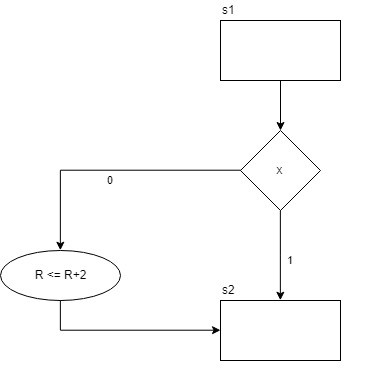
\includegraphics[scale=0.7]{ASMD1.jpg}
				\caption{Answer to state 1}
			\end{figure}
			\begin{figure}[H]
				\centering
				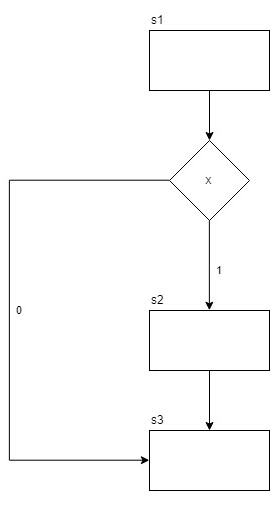
\includegraphics[scale=0.7]{ASMD2.jpg}
				\caption{Answer to state 2}
			\end{figure}
			\begin{figure}[H]
				\centering
				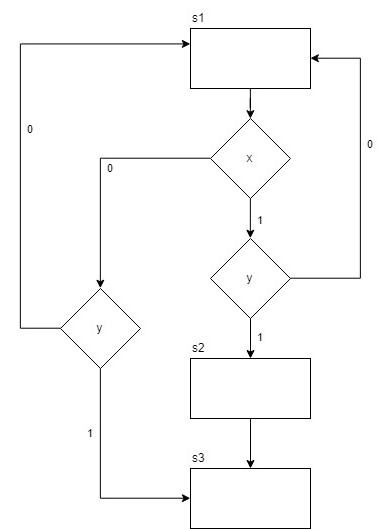
\includegraphics[scale=0.7]{ASMD3.jpg}
				\caption{Answer to state 3}
			\end{figure}	
		\item P2\\
			\begin{figure}[H]
				\centering
				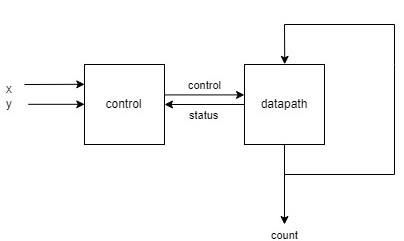
\includegraphics[scale=0.7]{Block-Diagram.jpg}
				\caption{Answer to state 1}
			\end{figure}
			\begin{figure}[H]
				\centering
				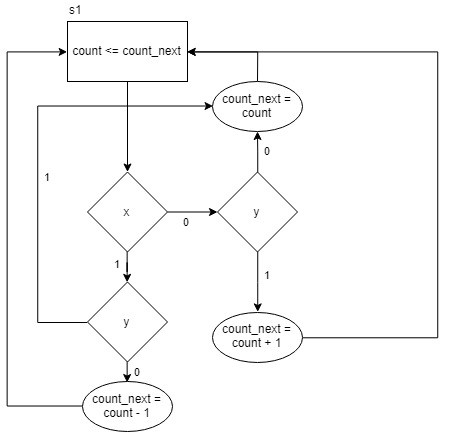
\includegraphics[scale=0.7]{ASMDCounter.jpg}
				\caption{Answer to state 2}
			\end{figure}
		\item P3 \\
			\begin{figure}[H]
				\centering
				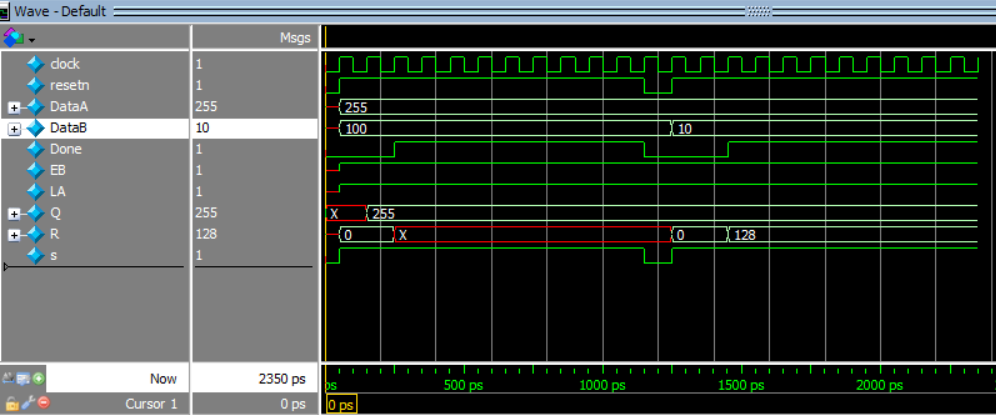
\includegraphics[scale=0.7]{divider-before.png}
				\caption{Non-working divider}
			\end{figure}
			\begin{figure}[H]
				\centering
				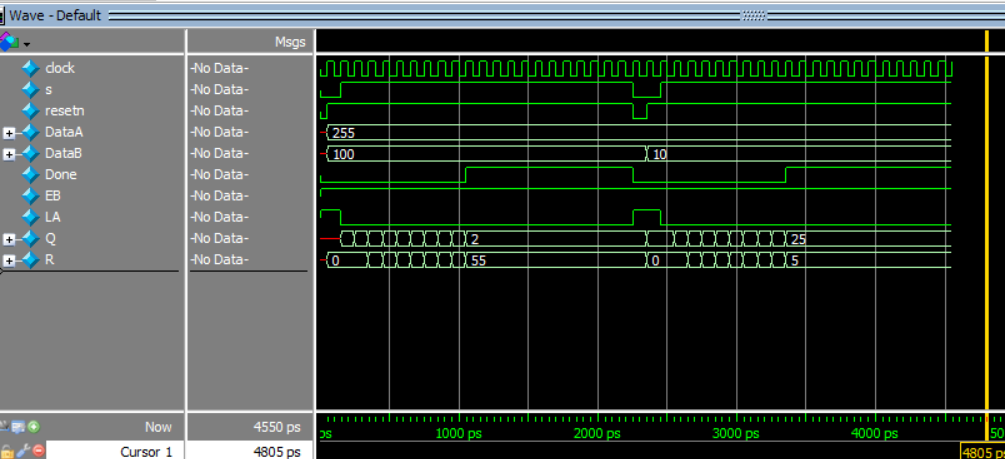
\includegraphics[scale=0.7]{divider-after.png}
				\caption{Working divider}
			\end{figure}
		\item Comments\\
		I like this homwork. I spent around 3 hours doing it. The major difficulty lies in understanding the shifter.
	\end{enumerate}
\end{document}
